\documentclass[sigconf]{acmart}

% Removes citation information below abstract
\settopmatter{printacmref=false}

%%
%% \BibTeX command to typeset BibTeX logo in the docs
\AtBeginDocument{%
  \providecommand\BibTeX{{%
    \normalfont B\kern-0.5em{\scshape i\kern-0.25em b}\kern-0.8em\TeX}}}





%% end of the preamble, start of the body of the document source.
\begin{document}

%%
%% The "title" command has an optional parameter,
%% allowing the author to define a "short title" to be used in page headers.
\title{Cryptography and system security -- Voting on GitHub pull request comments with Ethereum Smart Contracts}



%%
%% The "author" command and its associated commands are used to define
%% the authors and their affiliations.

\author{Jan-Erik Wieczorek}
\affiliation{%
 \institution{University of Applied Science}
 \city{Flensburg}
 \state{Schleswig-Holstein}
 \country{Germany}}
\email{jan-erik.wieczorek2@stud.hs-flensburg.de}
 
\author{Nick Johannsen}
\affiliation{%
 \institution{University of Applied Science}
 \city{Flensburg}
 \state{Schleswig-Holstein}
 \country{Germany}}
\email{nick.johannsen2@stud.hs-flensburg.de}



%%
%% The abstract is a short summary of the work to be presented in the article.
\begin{abstract}
As technologies such as blockchain and cryptocurrencies become more and more accepted in the general population, this opens up opportunities to be exploited. One of which is the possibility of a decentralized, unbiased voting mechanism for comments in the internet or more specific on GitHub. For that purpose we developed a solution, which is to be discussed in this paper.
\end{abstract}

\begin{CCSXML}
<ccs2012>
   <concept>
       <concept_id>10002978.10002979</concept_id>
       <concept_desc>Security and privacy~Cryptography</concept_desc>
       <concept_significance>500</concept_significance>
       </concept>
   <concept>
       <concept_id>10002951.10002952</concept_id>
       <concept_desc>Information systems~Data management systems</concept_desc>
       <concept_significance>500</concept_significance>
       </concept>
   <concept>
       <concept_id>10011007.10011074</concept_id>
       <concept_desc>Software and its engineering~Software creation and management</concept_desc>
       <concept_significance>100</concept_significance>
       </concept>
 </ccs2012>
\end{CCSXML}

\ccsdesc[500]{Security and privacy~Cryptography}
\ccsdesc[500]{Information systems~Data management systems}
\ccsdesc[100]{Software and its engineering~Software creation and management}



\keywords{Cryptocurrency, Chrome Extension, Ethereum, Blockchain, Sokol Testnet, POA, GitHub, Pull Request, Token, Token Curated Registry, Smart Contract}



%%
%% This command processes the author and affiliation and title
%% information and builds the first part of the formatted document.
\maketitle
\pagestyle{plain}



\section{Introduction}

\subsection{Development with GitHub}

GitHub is a platform that enables Developers to work on open-source projects together or alone. \cite{github} Open-Source development is a type of software development in which everyone (users, developers, maintainers) have access to the source code of a software. This makes working together and getting help from other users easier.\\

On GitHub you can find a lot of open-source software repositories which anyone can contribute to. GitHub implements Git, which is a version control protocol which allows to identify mistakes in code and in the worst case roll back to a previous state of the source code that is known to work. Contributors don’t have to fear breaking something and contributions will mostly be reviewed before they are taken into the repository. Those contributions are handled via pull requests. A contributor can post a pull request so mainainters of a repository can see that someone wants to contribute to the project.\\

A user on GitHub can start a repository for their software and push their code to it. Depending on the settings that the user opted for, this marks the start of an open-source project.
Now users can start pulling the source code, working on it and therefore adding their own changes to the software. Those changes can be proposed to the repository maintainer via a pull request.
On top of that GitHub implements features for users to give feedback on pull requests, open issues to report bugs in a software or leave general feedback/feature wishes to the software.\\

An example of open-source development on GitHub and users giving feedback to feature requests can be found on many repositories by GitHub itself.\\

While GitHub itself is not open-source, an alternative called GitLab is open source and its users are free to contribute ideas and feedback to it, though it lacks features which the much wider adopted platform GitHub offers its users. \cite{gitlab}\\


\subsection{Motivation}

With etiquette in the internet being in the state it is in today, one has to expect at least some degree of sabotage or toxicity when providing a platform for people to speak their minds. Unfortunately this is no exception for open source projects or comments in public GitHub repositories. This however is a quite dire situation since (the often unstructured) collaboration on complicated software projects requires at least some degree of cooperation.
This situation creates the need for a solution to somehow reduce obstructive comments without restricting them or providing some single individuals the means to do so.
Furthermore the comment section on issues, pull requests or commits often is quite bleak when in truth this is the place to discuss and therefore possibly find new solutions to improve the project. Meaning that there is some need to incentivise people to create and participate in those discussions.


\subsection{Goal}

As lined out in the previous chapter, the goal of beGit is for GitHub comments on pull requests to be more civil and helpful. We further want it to motivate more people in taking part in open source development and discussion. More participation in commenting on pull requests should result in a better software overall, since more discussion sparks the possibility for more ideas.

\subsection{Current State}

Currently the ability to redact and manage comments on GitHub lies completely with the repository owner and people they see fit to do so(https://docs.github.com/en/github/building-a-strong-community/moderating-comments-and-conversations). This creates the possibility of censoring unwanted opinions, critique or covering up ones own mistakes, therefore generating an unfair playing field for discussions by design. In any project that truly is open, every participant should be valued the same and have equal say when debating and judging comments.
However in its current state the only way for ordinary developers to assert some value to good comments or to punish bad ones, is to either point out those points in a comment of its own or to react to said comment with a variety of emotes. This approach provides neither incentive to write good comments nor does it grant the community the authority to manage itself.


\section{Solution}

\subsection{Idea}

The idea is to incentivise users on a repository to post good quality comments on pull requests to discuss the matter.
This can be done through voting. Imagine a user posting a comment and staking some ethereum on that comment. That ethereum can be used in a TCR (Token Curated Registry \cite{medium1}) to be obtainable by voters as prize money for voting. In a TCR the one posting something, in this case a comment, has to stake something of value with it. Other users can now vote for or against the post with their own ethereum. This disincentivises users from voting negatively on something they know would be good for the project and vise versa, because at the end the side (positive or negative) that had the most ethereum staked in their favor wins the staked ethereum from the losers side. The comment poster profits only when the comment has been voted positively.
With the incentive of making a profit, the users are incentivised to post good comments and vote with the projects future in mind.\\

On top of that the community now gains a visible guide on what is good for the project and what is not. In the case of an administrator not taking highly liked contributions into account, the community would leave the project, since it is now obvious what is liked and what is not.


\subsection{Protocol}

\begin{figure*}
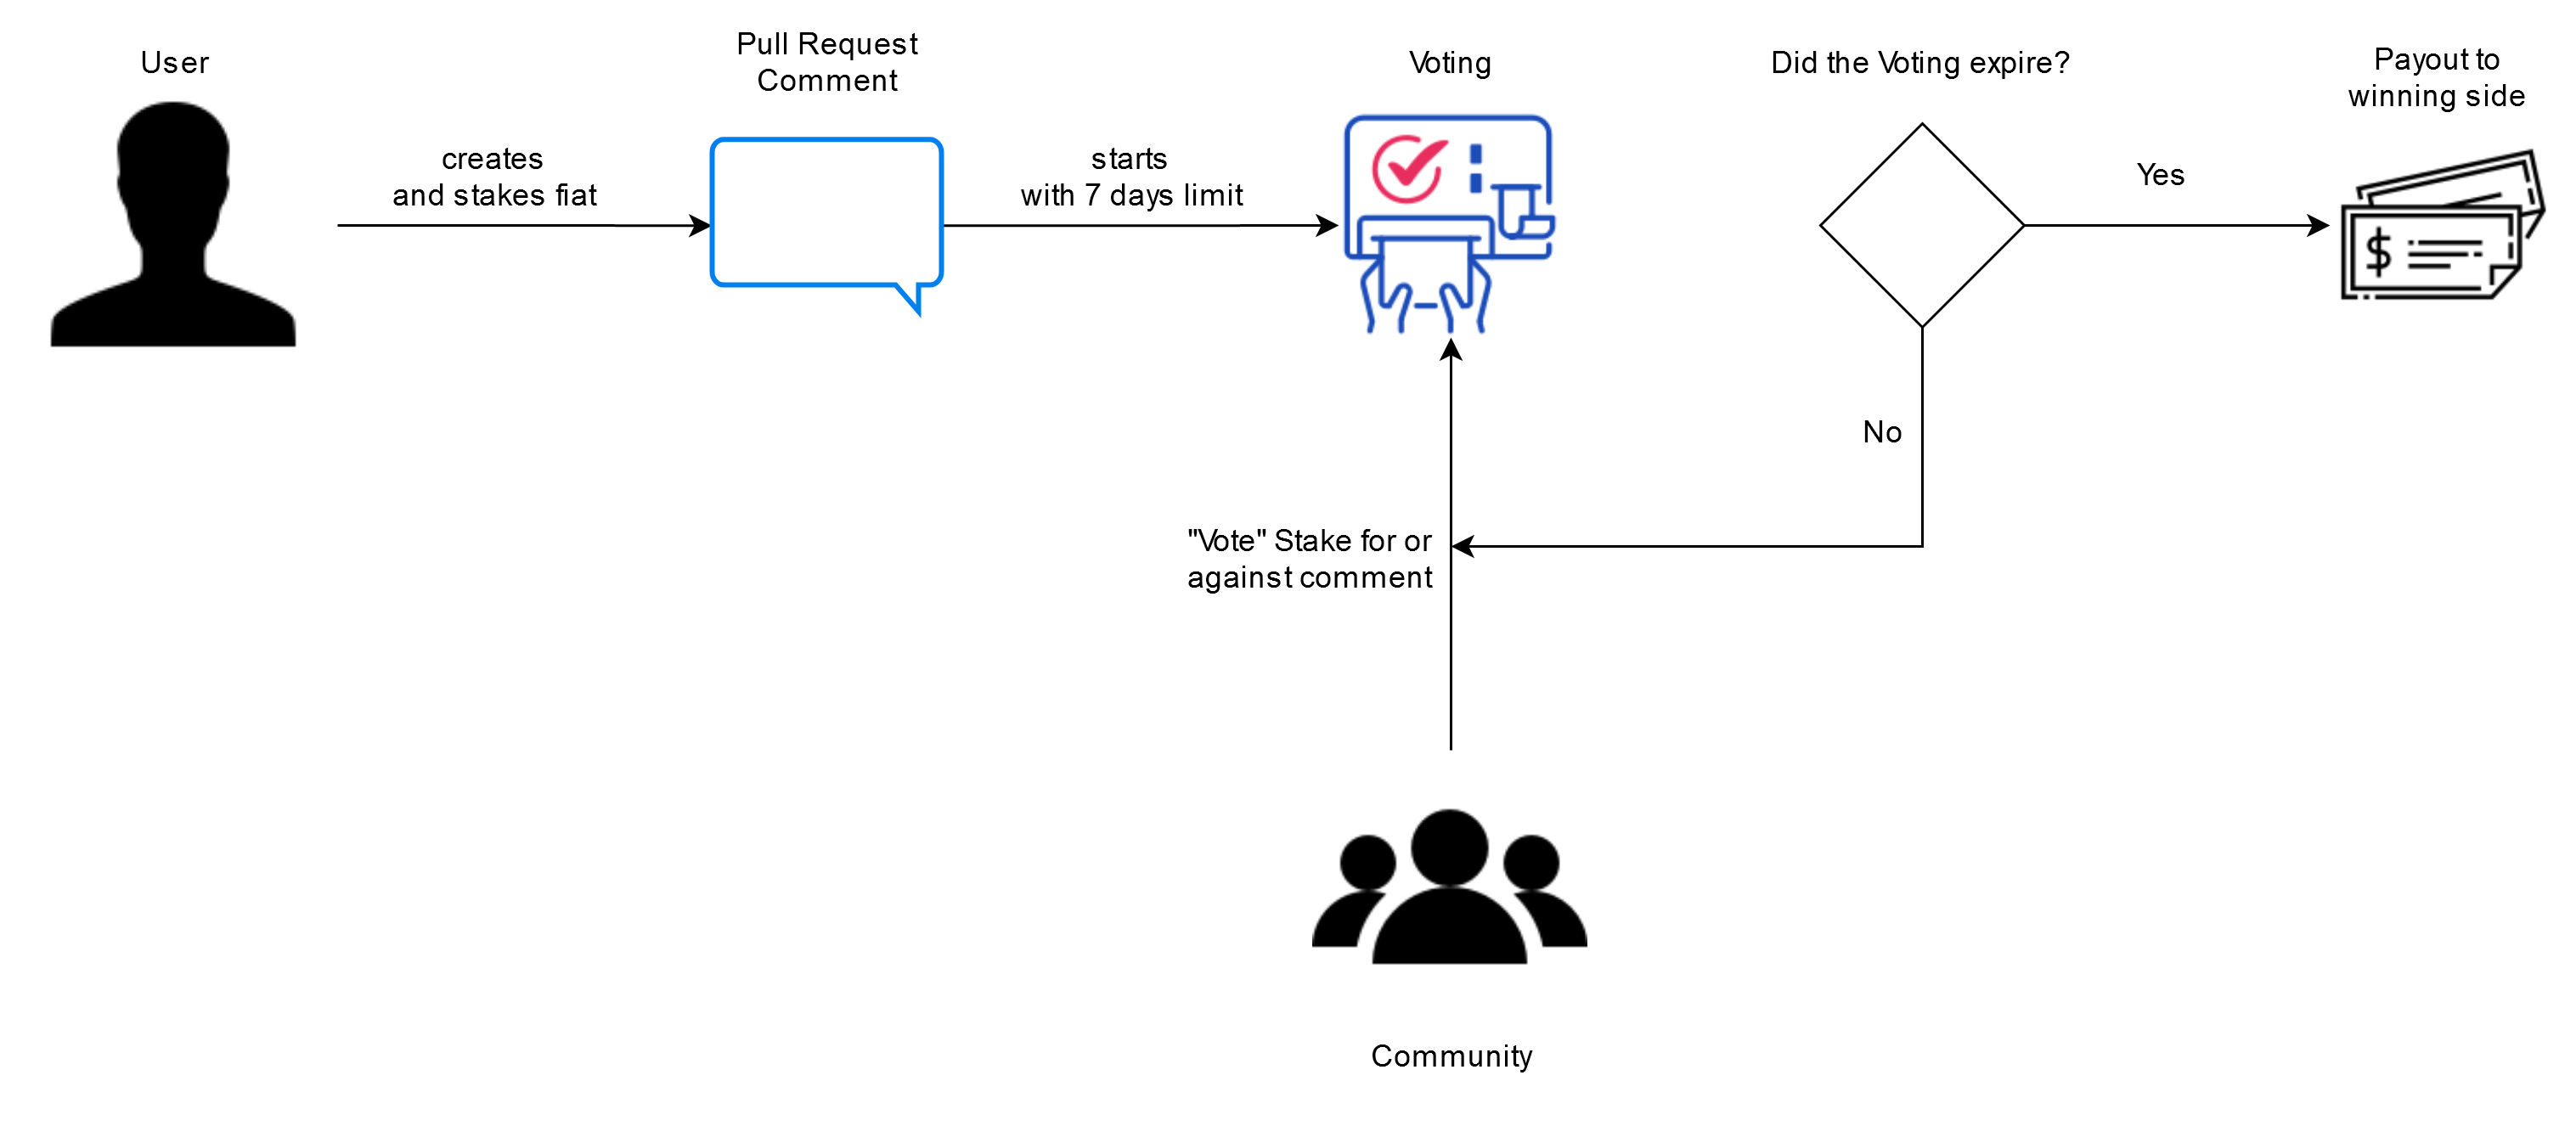
\includegraphics[width=\textwidth]{Protocol Grafik.png}
\caption{Graphic to illustrate protocol}
\label{fig:ds}
\end{figure*}

The protocol consists of a series of steps that happen in succession. This way it is easy for the users to comprehend and know at what stage in the protocol they are.
The protocol steps are:
\begin{itemize}
\item Initialization of the comment and staking process
\item Start the voting phase
\item Community members voting during the time period
\item The time period is over, calculating who won
\item Paying the winning side
\end{itemize}
The initialization part is done by the user who comments on the pull request. The user stakes some ethereum on the comment. The comment is now created in the TCR smart contract.\\

Starting the voting phase with a time limit ensures that after that time period the winning participants of the voting will receive their ethereum at some point.\\

After the voting phase starts, now that the comment has been posted as a staked comment, GitHub users will see the comment as votable.
Community members can either upvote or downvote a comment. They set the amount of ethereum they want to stake on their vote and are free to expand their stakes at any time during the time period in which voting is allowed, but not to withdraw to avoid possible mainpulation.\\

As soon as the time period for voting is over, users won’t have the ability to vote anymore. The smart contract will count the results and pay all the participants on the winning side with the ethereum in the pool. Every participant gets the percentage of the pool that they contributed to it.
The comment owner will receive a portion of the pools ethereum as well, in case the voting result is positive.


\subsection{Implementation}

Our implementation works with a chrome browser extension \cite{extensionDocs} and the ethereum blockchain.
The following sections will explain how we use ethereum smart contracts to manage comments on pull requests and a chrome browser extension to give users of GitHub a frontend to work with the smart contracts.


\subsubsection{Contracts}

Smart Contracts are one of the defining features of the ethereum blockchain and as such a short explanation is in order. To do that we recap, that a blockchain essentially is a way to store data. This data is chained together in blocks, hence the name blockchain. Each of these blocks then classically contains data of individual transactions between anonymous addresses. Each of those addresses represents a wallet, capable of holding some amount of cryptocurrency. Thus the blockchain stores the complete state the network currently is in, and ever was in. Smart Contracts however expand the capabilities of a blockchain significantly. Smart Contracts, as the name implies are a form of automated contract, stored and executed on the blockchain. Consequently a blockchain with Smart Contracts no longer just stores data, but also is able to do some computation. Additionally those Smart Contracts inherit the already existing features of a blockchain and are therefore decentralized, secure and verifiable while still being anonymous. However since computational power is not free and each contract is limited by the blocksize, Smart Contracts are not capable of highly sophisticated tasks, nor would you ever want to run one, since you pay a fee each time you execute a Smart Contract. This fee is proportional to the amount of computation, your transaction causes. The act of simply reading from a Smart Contract therefore is not associated with a fee.

Additionally we are working with the Sokol POA Testnet, which has no real value tokens. This testnet is for development purposes. Our smart contracts are deployed to that blockchain. \cite{sokolTestnet}

\paragraph*{First Iteration}

The initial approach to the creation of the Smart Contract, was to create a contract, containing the IDs of all registered comments as well as the corresponding votes and wallet addresses for each of them. This method however required some complex data structures and therefore needed quite a lot of memory within a single contract. In fact so much, that the contract became very convoluted and we reached the limitations of said contract. This resulted in a reorientation and led to a new approach.

\paragraph*{Second Iteration}

After the first, bloated iteration, the second followed a more methodical process and was targeting a cleaner, more concise outcome. To this end, the contract was split up into two different ones. One contract solely serves the purpose of saving all IDs of all registered comments. Additionally those IDs are mapped to addresses. Those addresses are in turn each the address to an instance of the second contract. The second contract then takes care of a single comment and is slightly more complex, than the first one. It stores the total value of all staked currency for and against the comment. Furthermore it holds addresses of all users who voted for or against the comment as well as their individual stake.
This more structured approach however complicates the process of writing and reading data slightly. Instead of having to call a single function from one contract and wait for the result, the extension now needs to first look up the comment in the first contract and then call whichever operation it wants to execute with the received address of the second one.
Nevertheless this minor inconvenience is a decent tradeoff for the increased clarity of the code greatly. Unfortunately though, there still is one major inconvenience, which can not be fixed. This is once again a matter regarding the complexity of operations within Smart Contracts. Once the voting on a comment expires, all stakeholder should be paid out their respective amount. To do that it is unavoidable to iterate over the whole list of all of them. However this is a task with varying complexity, depending on the total count of stakeholders. Therefore it can not be completed by the contract itself due to the inherent limitations of Smart Contracts. Consequently this is a task the extension will have to perform.


\subsubsection{Extension}

The creation of a Google Chrome extension is generally loosely analogous to that of a website. The code is written in javascript, which is used to create an interface with html/css or to manipulate the DOM of existing websites. Since our extension should integrate into GitHub sites it mostly does the latter. Additionally the extension provides a basic settings window, which creates its interface from scratch. The extension also requires some communication with the GitHub API. Each of those tasks is handled in a separate file, which are described in detail below.

\paragraph{Frontend}

The frontend is as integrated into the design of GitHub as possible and reuses some of its css-styling to blend in. To interact with the smart contract the extensions frontend presents the user some elements like a button to post a comment with stake, buttons to upvote or downvote on every comment that was posted with a stake and the remaining time period for the voting phase of the comment. When the time period for voting is expired, an additional button to start the payout process becomes available. Once it is clicked, the extension of the user who clicked it calls a method within the Smart Contract repeatedly. This method takes the next stakeholder, calculates their reward and transfers the calculated amount to them. The reasoning for this tedious process lies within the limitation of Smart Contracts and is explained in the previous chapter.

\paragraph{API Connections}

One critical point for the extension is, to make sure that there is no inconsistency between the comments saved and staked upon within the Smart Contract and on GitHub itself. To ensure that, the extension makes extensive use of the GitHub API. \cite{rest} It does so by providing a seperate button to post a registered comment. This button does not send the post via the website, instead the written comment gets extracted from the DOM, as well as all information about the current repository and issue. Those informations are then used to create an http message, which gets sent to the API, finally posting the comment.
Before any of that can happen, the extension needs to verify the user. This is done via Oauth2. \cite{oauth}

\paragraph{Settings}

The primary task of the settings is to provide the user with an interface to save the wallets they want to use for staking on comments. This data is saved within the Chrome storage, meaning it is even usable when the user is logged onto another system as long as they are logged into their Google account.


\section{Conclusion}

Following the testing of our browser extension with the ethereum blockchain, we are presenting some thoughts on how a browser extension can work for our goal and how the ethereum blockchain makes this possible. To that we will present issues that might arise due to the limitations of both technologies and what to look out for.

\subsection{Discussion}

There are multiple things we need to address for the ethereum blockchain, the chrome extension and how they work together.

\subsubsection{Ethereum Blockchain}

Interactions with the blockchain can be quite slow. There is a speed limit for the Extension to operate at, because of the ethereum blockchain. If a transaction has to be made immediately you need to pay a higher fee for it to be processed faster. That can be a problem, since there is also a limit on the fee, a maximum fee. Too many computations on a smart contract can hit the maximum fee limit of the blockchain.
Limitation with scaling to higher and higher counts of votes on a comment will then be limited by the speed thanks to the fee limit.


\subsubsection{Chrome Browser Extension}

Since the extension is doing a loop through all participants that need to be paid when the payout is initiated, this means that the payout is taking quite a while to finish, thanks to the slow interaction speed with the smart contract.
Not doing the payout process in the extension would be preferred.


\subsubsection{Extension and blockchain working together}

Like mentioned before, the speed of the interactions between the extension and the smart contract is an issue that we need to deal with, because of the chosen architecture.
We propose a third party, like a custom server, that acts as a middleman between the extension and the smart contract, because the extension stops the payout process once the tab is being refreshed. This does not break the payout chain, it just stops it. The next time a client will start the payout it will start where it left off. But assuming a large number of votes this could take a long time to finish.


\subsubsection{Was the goal achieved?}

The goal could be seen as achieved, in the definition that a proof of concept was built and works. It demonstrates that it can work but it also shows the flaws of this approach, as mentioned before.\\

We can not say for sure if the application in a field test with multiple users and actual ethereum that has real world value would work as intended. By running it only on a testnet we know only that the proof of concept works.


\subsection{Future prospects}

A project for the future could be to build a server that can act as a buffer for commands to the smart contract. Those are still being sent from the client, at the moment. IIn addition to that the extension would need to communicate with the server instead of the web3.js library that is currently used. \cite{web3} The proposition is, that the client will send a command to the server on what has to happen with the smart contract, receiving data or changing data. This would have a huge benefit for the payout phase, since the client needs to stay waiting in the current tab until the payout is done, as it is now. The server could loop through all commands to the smart contract, once a client says that the payout needs to be started. That leaves the client independent of the payout.\\

Another idea would be to not restrict the voting to pull request comments. Allowing users to vote everywhere on GitHub where there are comments could be useful. The effects on how complex the usage for the user is going to be would have to be investigated.\\

Since the quality of comments and vote is a concern knowledge tokens (implementing a knowledge-extractable voting (KEV) protocol \cite{medium2}) could be introduced to the protocol. A knowledge token represents a user's knowledge on software development.
Those tokens could be staked and weigh the ethereum tokens.
Knowledge tokens could be obtained by a quiz or by contributing code to a project.
Once a user has knowledge tokens they can weigh their ethereum a lot higher by staking those alongside the ethereum tokens, therefore having a lot more influence on voting than users without knowledge tokens who just want to participate with their amateur opinion (form the point of view of the protocol it would be considered amateurish).\\

As for the extension itself, up to this point it has been built with being a proof of concept in mind. There is room for improvement for the frontend design and some quality of life features.
For example the implementation of how the users are voting could be separated more from the actual comment text.\\ 


%%
%% The next two lines define the bibliography style to be used, and
%% the bibliography file.
\bibliographystyle{ACM-Reference-Format}
\bibliography{references}


\end{document}
\endinput
%%
%% End of file `sample-sigconf.tex'.
